% Prof. Dr. Ausberto S. Castro Vera
% UENF - CCT - LCMAT - Curso de Ci\^{e}ncia da Computa\c{c}\~{a}o
% Campos, RJ,  2022
% Disciplina: Paradigmas de Linguagens de Programa\c{c}\~{a}o
% Aluno: Rômulo Souza Fernandes



\chapter{ Introdução}

O Python é uma linguagem orientada a objetos de alto nível, que possui uma sintaxe simples e objetiva, assim colaborando para a fácil compreensão do código-fonte e permitindo que a linguagem seja produtiva. O Python contém várias estruturas de alto nível, como hora, data, dicionários, listas, complexos, entre outras estruturas, contém um amplo conjunto de módulos disponíveis para utilização, frameworks que podem ser acrescentados, possui ferramentas de outras linguagens atuais, como persistência, unidades de teste, geradores, introspecção e metaclasse, além de ter disponíveis diversas bibliotecas, como IPython, Matplotlib, mIPy, NumPy, Pandas, SciPy, ScraPy, entre outras bibliotecas conhecidas.

O Python é uma linguagem multiparadigma, suportando a programação orientada a objetos, modular e funcional. A linguagem Python foi criada na Holanda, no ano de 1990, por Guido van Rossum, no Instituto Nacional de Pesquisa para Matemática e Ciência da Computação. \cite{Borges2014}

A linguagem Python é de código aberto, porém o criador Guido van Rossum possui a função central de decidir a evolução da linguagem. O Python se popularizou e se tornou a linguagem de desenvolvimento de aplicações mais indicada para iniciantes, assim sendo aconselhada como primeira linguagem de programação. \cite{Perkovic2016}

%\begin{quote}

%\end{quote}


\section{História da linguagem Python}

O intuito de Guido van Rossum era criar uma linguagem que pudesse suprir suas exigências, assim criando o Python, com base na linguagem ABC, mas solucionando as incoerências encontradas por ele na linguagem. O Python tinha como usuários principais os engenheiros e físicos.


A seguir um pouco da história da linguagem Python, baseados em \cite{Perkovic2016} e \cite{Borges2014} :
\begin{itemize}
  \item O Holandês Guido van Rossum foi o autor principal da linguagem Python. O autor trabalhava no CWI (Centrum Wiskunde \& Informatica), localizada em Amsterdã na Holanda.
  \item  O nome Python não veio da espécie de serpente e sim do seriado de comédia preferido do autor da linguagem, chamado Monty Python's Flying Circus.
  \item A versão 0.9.0 do Python foi lançado em 1991, incluindo manipulação de exceções, classes, listas e strings. Incluia também alguns aspectos de programação funcional como lambda, maps, filter e reduce.
  \item  No ano de 1995, o autor da linguagem continuou seu trabalho sobre Python na Corporation for National Research Initiatives (CNRI) em Reston, Virginia, USA.
  \item  Em Maio de 2000, Guido van Rossum e o grupo de desenvolvimento do Python se mudaram para BeOpen.com, assim formando a equipe BeOpen PythonLabs.
  \item A versão 1.6 do Python foi lançada em 5 de setembro de 2000.
  \item A versão 2.0  do Python foi lançada em 16 de outubro de 2000.
  \item A versão 3.0 do Python foi lançada em 3 dezembro de 2008.
  %\item A última versão lançada do Python é a versão 3.12, lançada em 4 de setembro de 2022
\end{itemize}

%Algumas linguagens s\~{a}o consideradas  tradicionais e outras s\~{a}o consideradas modernas (ver Fig.\ref{afp}). Devemos observar aqui, que a inclus\~{a}o de qualquer figura, significa que ela deve ser referenciada em algum lugar do texto
%   \begin{figure}[H]
	%   \begin{center}
     %   \caption{Logos da Linguagem Python} \label{ling1}
      %  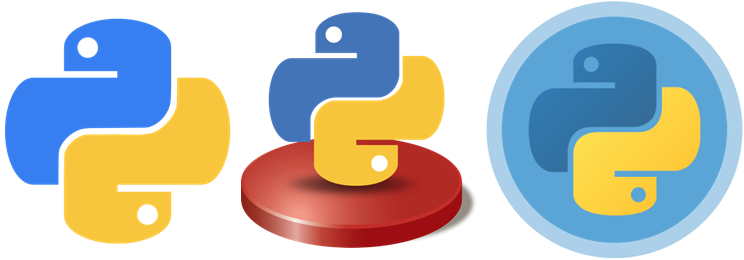
\includegraphics[width=12cm]{Python01.png} \\
       % {\tiny \sf Fonte: O autor deste trabalho }
    %\end{center}
   %\end{figure}

%Algumas figuras s\~{a}o criadas o elaboradas pelo mesmo autor, neste caso, deve-se escrever como fonte "O autor", "Os autores", etc. Figuras que incluam imagens de outras fontes deve-se especificar claramente, indicando o link o referencia correspondente, por exemplo, uma imagem que aparece em \cite[p. 93]{Sprankle2012}, \'{e} mostrada na Fig.\ref{afp} e a fonte deve ser indicada na parte inferior da figura.
   %\begin{figure}[H]
    %\begin{center}
        %\caption{Algoritmo, Diagrama de fluxo, e Pseudo-código} \label{afp}
        %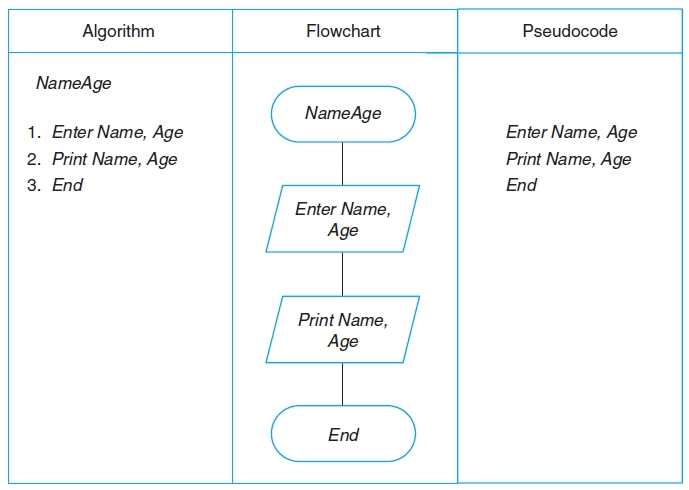
\includegraphics[width=10cm]{afp.jpg} \\
        %{\tiny \sf Fonte: \cite[p. 93]{Sprankle2012} }
    %\end{center}
   %\end{figure}

   \section{Áreas de Aplicação da Linguagem}
   O Python está entre as linguagens de programação mais utilizadas no mundo, é utilizado por usuários individuais, mas sua aplicação se estende para empresas reais. A natureza do Python é de propósito geral, assim tornando a linguagem aplicável em quase todas as áreas. A IBM, Seagate e Hewlett-Packard, que utilizam o Python para testes de hardware. O Yahoo! e Google usam a linguagem em serviços de Internet. Já a empresa Industrial Light and Magic e outras empresas de filmes utilizam o Python na produção de animações. Entre todas as aplicações para o Python atualmente, o ponto em comum é que a linguagem é usada em todo o espectro, em questão de domínios de aplicação. \cite{Lutz2007}

        \subsection{Big Data}
        Atualmente o Python é uma das melhores linguagens de programação para trabalhar com Big Data. Um dos motivos dessa preferencia de uso é, o suporte avançado de inúmeras bibliotecas e frameworks, muitas das bibliotecas são voltadas para lidar com Big Data, dando suporte e auxiliando na implementação  de algoritmos de Machine Learning e Data Analytics. Abaixo algumas das bibliotecas de software livre:
        \begin{itemize}
        	\item SciPy: Utilizada para computação técnica e computação científica, possibilita a interpolação, otimização, integração e modificação de dados utilizando funções especiais, álgebra linear, etc.
        	
        	\item NumPy: Utilizada para computação numérica para dados com formas de grandes matrizes multidimensionais e arrays. A biblioteca também oferece diversas funções matemáticas de alto nível, para manipular os dados com transformada de Fourier, álgebra linear, processamento de números aleatórios, etc.
        	
        	\item Scikit-learn: Utilizada para Machine Learning, relacionado a vários algoritmos de regressão, clustering e classificação. Pode ser utilizado também em conjunto com outras bibliotecas, como a NumPy e SciPy.
        	
        	\item Pandas: Utilizada para análise e manipulação de dados, oferece diversas estruturas de dados e operações para manipulação de dados, no formato de séries temporais e tabelas numéricas. A biblioteca também dispõe diferentes ferramentas para gravar e ler dados, entre estruturas de dados na memória e diferentes formatos de arquivo.
        \end{itemize}
        
        O Python possui uma sintaxe simples, possibilitando uma fácil leitura do código, assim tanto os estudantes iniciantes quanto os desenvolvedores experientes, podem se concentrar melhor no objetivo ao invés de se desgastar se concentrando nas nuances técnicas da linguagem que está utilizando. Sendo assim, a linguagem preferida dos Cientistas de dados e Engenheiros de Big Data. 
        
        A linguagem Python é extremamente flexível, permitindo finalizar mais trabalhos com menor número de linhas de código. O Python também é escalável na manipulação de dados em grandes quantidades, sendo um ponto muito importante quando se trata de Big Data. Comparando o Python com outras linguagens de programação utilizadas em Big Data Analytics, como R e Java, não são tão escaláveis e flexíveis como o Python, onde se o volume de dados aumentar, o Python sem dificuldades pode aumentar a velocidade de processamento dos dados, sendo uma tarefa complicada para fazer em R ou Java. \cite{McKinney2019}

        \subsection{Orientação a objetos}  
        O Python é uma linguagem multiparadigma, suportando diferentes abordagens de programação, um jeito de solucionar problemas de programação é criar objetos, esse método é conhecido como Programação Orientada a Objetos(POO) e a orientação a objetos é um dos paradigmas da linguagem Python, com isso, a criação de objetos e classes é mais simples. 
        
        No Python os dados são guardados em objetos, em outras linguagens, determinados tipos são guardados na memória, não em entidades abstratas como objetos. A programação orientada a objetos é um importante método de organizar e desenvolver códigos, focando em criar códigos reutilizáveis. \cite{Lutz2007}
        
        No Python, a programação orientada a objetos possui alguns pontos importantes, baseados no mesmo autor do parágrafo anterior: 
        \begin{itemize}
        	\item Encapsulamento: Restrição ao acesso de métodos e atributos de uma classe, evitando que os dados sejam alterados diretamente, na linguagem Python existe apenas o private e public.
        	
        	\item Métodos: São funções definidas no corpo da classe. Utilizados para definir o comportamento do objeto. 
        	
        	\item Objeto: É a instância de uma classe. Somente a definição do objeto é definida no momento que a classe é definida.  Consequentemente nenhum espaço de memória é alocado.
        	
        	\item Classe: Juntam as funcionalidades de um certo objeto, servindo como um modelo.
        	
        	\item Polimorfismo: É a capacidade de utilizar uma interface para vários tipos de dados. Possibilitando que o objeto possua o poder de assumir diversas formas. 
        	
        	\item Herança: Cria uma classe nova que será descendente e irá utilizar particularidades de outra classe já existente, sem realizar modificações na mesma.
        	 
        	
        \end{itemize}


        \subsection{Pentest} 
        O Python está entre as melhores linguagens para pentest e segurança da informação, isso é devido a grande quantidade de bibliotecas, ferramentas, frameworks, versatilidade, ser multiplataforma, entre outros pontos que tornam o Python uma das melhores linguagens para essa aplicação, como código de fácil leitura e sintaxe simples. A linguagem é usada para diversas finalidades dentro do processo, possibilitando que as soluções sejam vinculadas e automatizadas sem dificuldades, como decodificar e enviar pacotes, varrer redes e portas, analisar malwares, acessar servidores, com base em \cite{Moreno2018} e \cite{Seitz2015}.
        
        Como citado, a linguagem Python possui uma grande diversidade de ferramentas, de acordo com os mesmos autores do parágrafo anterior, essas são algumas das ferramentas disponíveis:
        \begin{itemize}
        \item Análise de malware:
        	\begin{itemize}
        		\item Exefilter: Utilizada para filtrar  tipos de arquivos para páginas web, e-mails e arquivos, podendo detectar diversos tipos de arquivos e apagar o conteúdo ativo.
        		
        		\item PyClamAV: Acrescenta a detecção de vírus maliciosos nas ferramentas do Python.
        		
        		\item Pyew: Utilizado geralmente para analisar malwares, o pyew desmonta e edita hexadecimais de linha de comando.
        	\end{itemize}
        
        \item Utilitários de rede:
        	\begin{itemize}
        		\item Dpkt: Utilizado para gerar e analisar pacotes de dados utilizando definições do protocolo TCP/IP.
        		\item Spoodle: Usado para verificar subdomínios e vulnerabilidade.
        		\item Knock Subdomain Scan: utilizado para retornar a lista de subdomínios do domínio de destino através da técnica de lista de palavras.
        	\end{itemize}
        
        \item Explorar bibliotecas:
        	\begin{itemize}
        		\item Scapy: Biblioteca e ferramenta de processamento de pacotes, podendo decodificar diversos protocolos, enviar pela rede, capturar e combinar respostas e solicitações. Oferece funções como as funções oferecidas pelo Tcpdump, Wireshark e Nmap, também oferece acesso programático.
        		
        		\item Python Nmap: Usado para analisar os resultado da varredura do Nmap e lançar ataques particularizados contra hosts específicos.
        		
        		\item Monda: O Monda é um depurador de imunidade, que auxilia no desenvolvimento de programas de exploração.
        		
        	\end{itemize}
        
        \item Forense
        	\begin{itemize}
        		\item Rekall: O Rekall é um framework criado pelo Google para realizar varreduras e análises de memória.
        		
        		\item LibForensics: É uma biblioteca para desenvolvimento de aplicativos Forenses digitais
        		
        		\item Aft: É um pacote de ferramentas forenses voltado para Android.
        		
        	\end{itemize}
        \end{itemize}
    
   
    	